\begin{minipage}{0.45\textwidth}
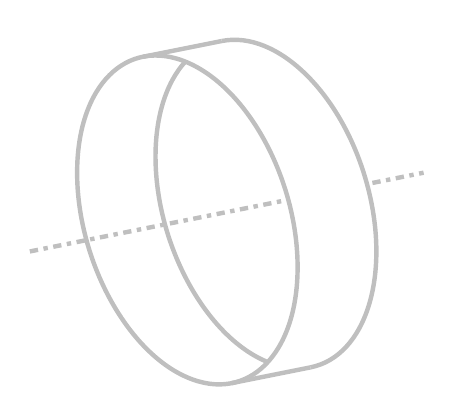
\begin{tikzpicture}
    \begin{scope}[x={(.7cm,-.3cm)},z={(-.5cm,-.1cm)}]
        \path (1,0,0);
        \pgfgetlastxy{\cylxx}{\cylxy}
        \path (0,1,0);
        \pgfgetlastxy{\cylyx}{\cylyy}
        \path (0,0,1);
        \pgfgetlastxy{\cylzx}{\cylzy}
        \pgfmathsetmacro{\cylt}{(\cylzy * \cylyx - \cylzx * \cylyy)/ (\cylzy * \cylxx - \cylzx * \cylxy)}
        \pgfmathsetmacro{\ang}{atan(\cylt)}
        \pgfmathsetmacro{\ct}{2/sqrt(1 + (\cylt)^2)}
        \pgfmathsetmacro{\st}{\cylt * \ct}
        %\fill[red!10] (\ct,\st,0) -- ++(0,0,-8) arc[start angle=\ang,delta angle=180,radius=1] -- ++(0,0,8) arc[start angle=\ang+180,delta angle=-180,radius=1];
        %\fill[red!20] (0,0,-4) circle[radius=1.03];
        \begin{scope}[every path/.style={ultra thick,black!25}]

            % front ellipse
            \draw (0,0,0) circle[radius=2];

            % arrows
            %\draw[-] (-.02,0,0) -- (1,0,0);
            %\draw[-] (0,-.02,0) -- (0,1,0);
            %\draw[dashed] (0,0,-8) -- (0,1,-8);
            %\draw[dashed] (0,0,-8) -- (1,0,-8);

            % middle ellipse
            %\draw (\ct,\st,-4) arc[start angle=\ang,delta angle=180,radius=1];
            %\draw[dashed] (\ct,\st,-4) arc[start angle=\ang,delta angle=-180,radius=1];

            % central axis
            \draw[dash dot] (0,0,4) -- (0,0,-2.5);
            \draw[dash dot] (0,0,-4.7) -- (0,0,-6);

            % measurement marker in middle of central axis
            %\draw[dashed] (-1,0,-4) -- (1,0,-4);
            %\draw[dashed] (0,-1,-4) -- (0,1,-4);
            %\draw[-][red] (-.2,0,-4) -- (.2,0,-4);
            %\draw[-][red] (0,-.2,-4) -- (0,.2,-4);

            % measurement line
            %\draw[->][red] (0,0,-4) -- (0,1,-4);
            %\draw[->][red] (0,0.5,-4) -- (0,1,-4);

            % Cylinder Edges
            \draw (\ct,\st,0) -- ++(0,0,-2);
            \draw (-\ct,-\st,0) -- ++(0,0,-2);

            % back ellipse
            \draw (\ct,\st,-2) arc[start angle=\ang,delta angle=180,radius=2];
            %\draw[red] (\ct,\st,-2) arc[start angle=\ang,delta angle=-23,radius=2];
            %\draw[dashed] (\ct,\st,-2) arc[start angle=\ang,delta angle=-20,radius=2];
            \draw[yshift=0.07cm,xshift=-0.55cm] (\ct,\st,-2) arc[start angle=\ang-23,delta angle=-134,radius=2];
        \end{scope}
    \end{scope}
\end{tikzpicture}
\end{minipage}
\begin{minipage}{0.45\textwidth}
\begin{tikzpicture}
    % Cylinder, Side View
    \draw[dash dot] (0,0) -- (3,0);

    \draw (1,-2) -- (1,2) -- (2,2) -- (2,-2) -- cycle;

    \draw[dashed,arrows={Stealth-Stealth}] (0.7,0) -- (0.7,1) node[left]{$a$} -- (0.7,2);
    \draw[dashed,arrows={Stealth-Stealth}] (1,2.3) -- (1.5,2.3) node[above]{$b$} -- (2,2.3);

    % Two Separate Circles
    \draw[dash dot] (4,0) -- (5,0);
    \draw (4.3,-2) -- (4.3,2);
    \draw (4.7,-2) -- (4.7,2);
    \draw[dashed,arrows={Stealth-Stealth}] (4.3,2.3) -- (4.5,2.3) node[above]{$d$} -- (4.7,2.3);
\end{tikzpicture}
\end{minipage}
